% NewsScope Report — CVPR-format NLP class project
% Compile with: pdflatex main && bibtex main && pdflatex main && pdflatex main

\documentclass[10pt,twocolumn,letterpaper]{article}

% \usepackage{cvpr}              % camera-ready
% \usepackage[review]{cvpr}      % anonymous review version
\usepackage[pagenumbers]{cvpr}   % page numbers (for submission / sharing)

%% preamble.tex — additional packages for NewsScope report

%%
%% Inline annotations (red TODO markers, disable for final version)
%%
\newcommand{\red}[1]{{\color{red}#1}}
\newcommand{\todo}[1]{{\color{red}#1}}
\newcommand{\TODO}[1]{\textbf{\color{red}[TODO: #1]}}
%% Disable for final submission:
% \renewcommand{\TODO}[1]{}
% \renewcommand{\todo}[1]{#1}

%%
%% Professional table rules (toprule / midrule / bottomrule)
%%
\usepackage{graphicx}
\graphicspath{{figures/}}
\usepackage{booktabs}
\usepackage{tabularx}
\usepackage{placeins}

%%
%% Multi-panel figures
%%
\usepackage{subcaption}

%%
%% Better math support
%%
\usepackage{amsmath}

%%
%% Paragraph spacing tweak (optional — enable near final version)
%%
% \renewcommand{\paragraph}[1]{\vspace{.5em}\noindent\textbf{#1.}}


\definecolor{cvprblue}{rgb}{0.21,0.49,0.74}
\usepackage[pagebackref,breaklinks,colorlinks,allcolors=cvprblue]{hyperref}

\def\paperID{00001}
\def\confName{ITCS 4111}
\def\confYear{2026}

\title{NewsScope: A Multi-Dimensional NLP Pipeline for News Genre Classification,
       Keyword Extraction, and Sentiment Analysis}

\author{%
Max Larsson\thanks{All authors contributed equally.}\textsuperscript{1},\;
Kamon Whiteside\footnotemark[1]\textsuperscript{1},\;
Ben Zou\footnotemark[1]\textsuperscript{1}\\[4pt]
{\small
\textsuperscript{1}University of Cantabria, Santander, Cantabria, Spain}\\
{\tt\small \{mlarsson, kwhit160, bzou\}@cantabria.es}
}

\begin{document}
\maketitle

\begin{abstract}
We present a multi-task NLP pipeline for automatic analysis of BBC News articles. The system addresses three complementary problems: genre classification, keyword and named-entity extraction, and sentiment analysis. Genre classification is performed by a custom Multinomial Naive Bayes classifier trained on the BBC News corpus \cite{greene2006practical}, achieving 98.24\% accuracy across five categories (business, entertainment, politics, sport, and technology) on the held-out test set. Keyword extraction combines TF-IDF ranking with part-of-speech filtering and NLTK's named-entity chunker \cite{bird2009natural}. Sentiment analysis uses a second Naive Bayes model trained on BBC articles pseudo-labeled by the VADER rule-based analyzer \cite{hutto2014vader}, keeping the sentiment model in-domain with the news register. The full pipeline is demonstrated live on a BBC RSS feed. These results suggest that bag-of-words Naive Bayes is a strong baseline for news genre classification, while sentiment analysis remains harder in this domain because news articles are often neutral and fact-driven.
\end{abstract}

\section{Introduction}
\label{sec:intro}

The volume of news produced online every day is staggering. Readers, researchers, and media organizations alike need ways to quickly understand what a given article is about, as well as if the article's tone is overall positive or negative. Doing this manually at scale is simply not feasible, which makes automated news analysis a practically important problem and a rich domain for applying NLP techniques.

Genre classification, where a topic category such as \textit{sport} or \textit{technology} is assigned to an article, is the most fundamental of these tasks. Beyond this, two additional layers of information are particularly useful: (1) the specific terms and entities that distinguish an article from the background corpus, and (2) the overall sentiment of the coverage, which can reveal editorial tone or public mood around a topic.

This project builds an end-to-end pipeline, which we call \textbf{NewsScope}, that addresses all three tasks within a shared workflow:

\begin{enumerate}
    \item \textbf{Genre classification:} A Multinomial Naive Bayes classifier assigns each article to one of five BBC categories.
    \item \textbf{Keyword and entity extraction:} TF-IDF scoring, POS-tag filtering, and named-entity recognition surface the most important terms and real-world entities in each article.
    \item \textbf{Sentiment analysis:} A Naive Bayes sentiment model trained on in-domain BBC data (pseudo-labeled by VADER) is compared against VADER's rule-based scores directly.
\end{enumerate}

\begin{figure*}[t]
\centering
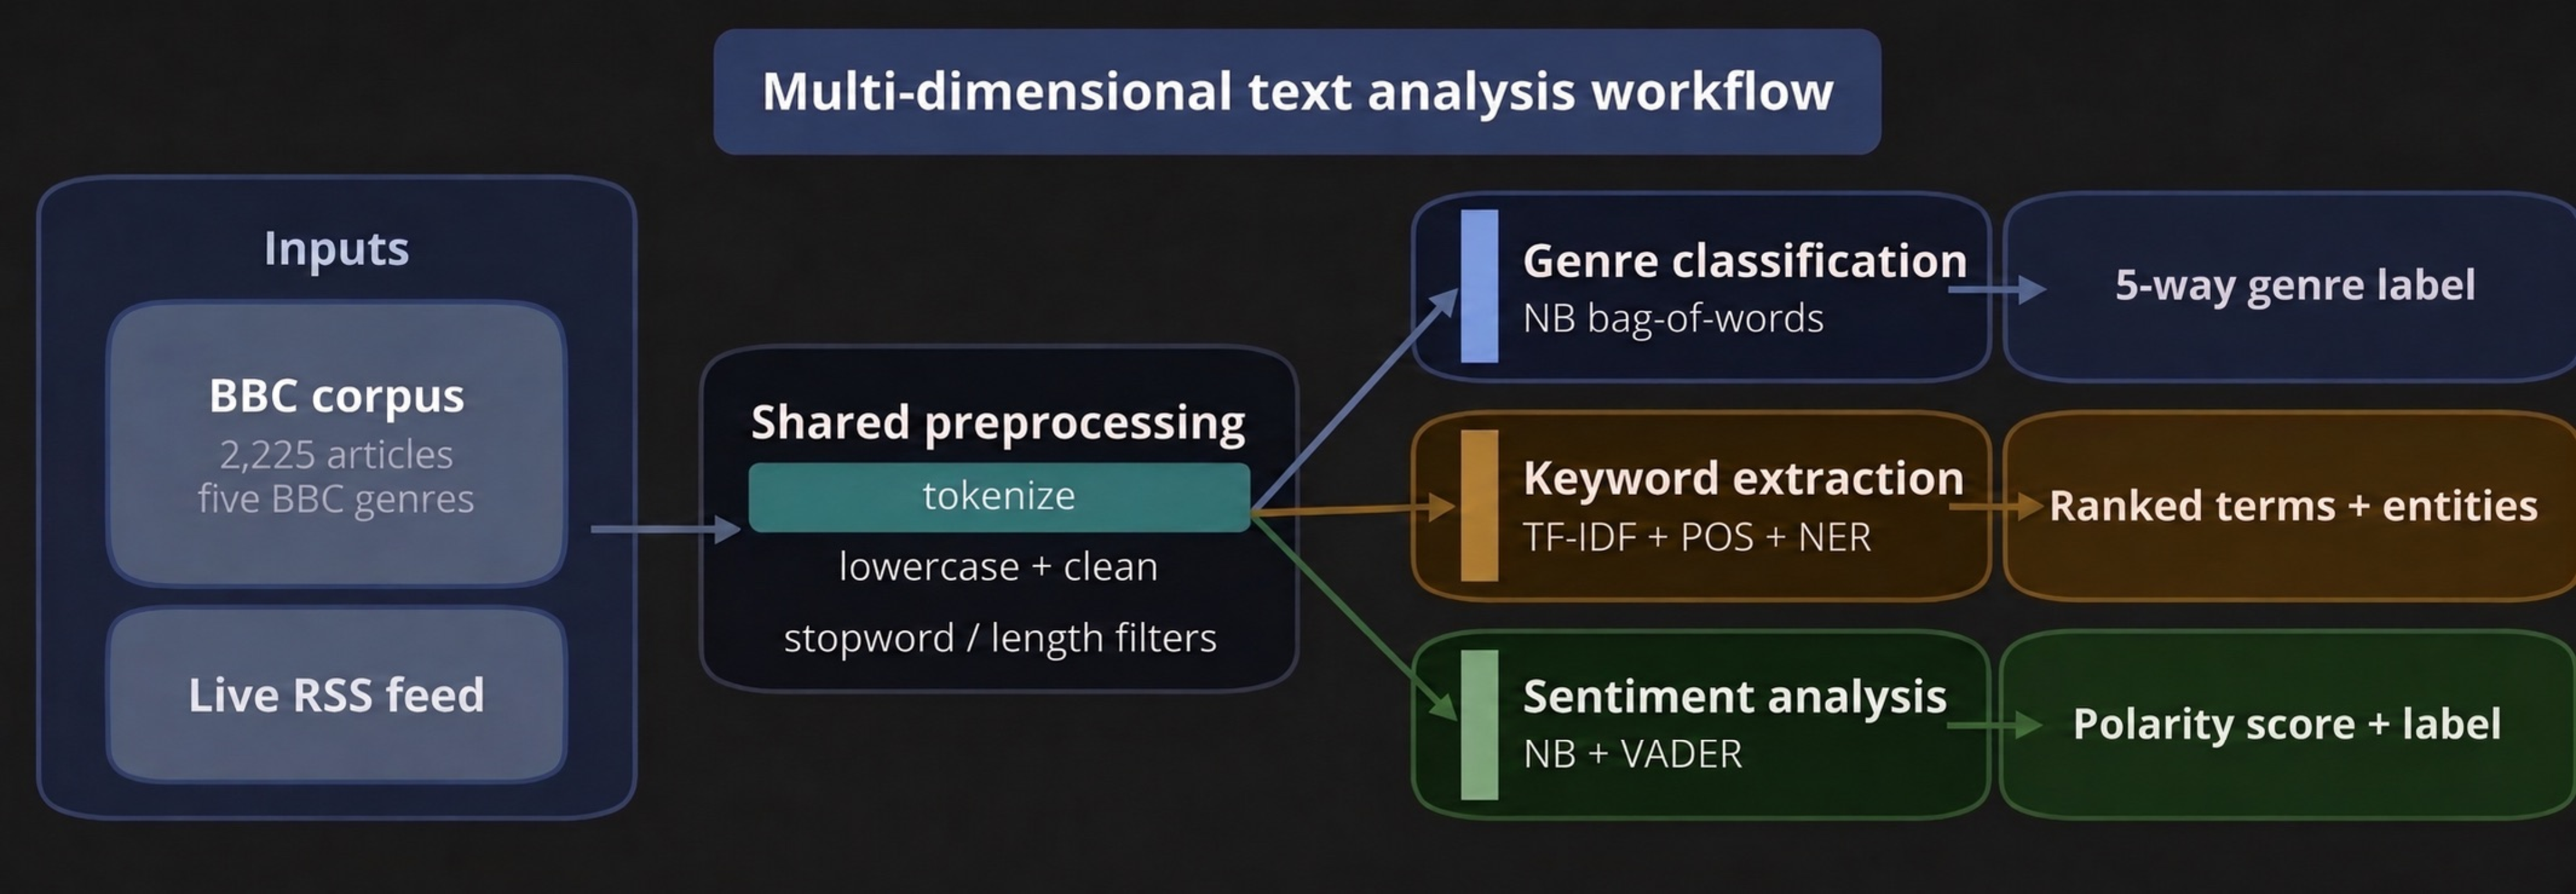
\includegraphics[width=\textwidth]{pipeline_architecture}
\caption{NewsScope pipeline overview. BBC articles and live RSS feed share one preprocessing stage before branching into genre classification, keyword/entity extraction, and sentiment analysis.}
\label{fig:pipeline}
\end{figure*}

The entire pipeline is implemented using NLTK \cite{bird2009natural} and scikit-learn, and demonstrated on live BBC RSS headlines.

\section{Data}
\label{sec:data}

\subsection{BBC News Corpus}
We use the BBC News dataset introduced by \citet{greene2006practical}, a widely-used benchmark for topic classification. The corpus contains 2,225 news articles collected from the BBC website between 2004 and 2005, spanning five editorial categories: \textit{business}, \textit{entertainment}, \textit{politics}, \textit{sport}, and \textit{tech}. The category distribution and exact split counts are shown in Table~\ref{tab:dataset}.

The articles are relatively short (median length approximately 300 words), topically diverse within each category, and written in a formal news register. Because BBC articles are carefully edited, the corpus has relatively few typos or non-standard forms, which simplifies preprocessing.

\subsection{Train / Validation / Test Split}

We apply a stratified split to preserve the class distribution in every partition. The dataset is divided into 80\% training, 10\% validation, and 10\% test, yielding 1,777 training, 221 validation, and 227 test articles. Stratification ensures that even the smaller categories (entertainment, tech) are adequately represented in every partition. The random seed is fixed at 42 for reproducibility.

\begin{table}[!htbp]
\centering
\small
\setlength{\tabcolsep}{3.8pt}
\begin{tabular}{lccccc}
\toprule
\textbf{Category} & \textbf{Articles} & \textbf{Share (\%)} & \textbf{Train} & \textbf{Val.} & \textbf{Test} \\
\midrule
Business      & 510 & 22.9 & 408 & 51 & 51 \\
Entertainment & 386 & 17.3 & 308 & 38 & 40 \\
Politics      & 417 & 18.7 & 333 & 41 & 43 \\
Sport         & 511 & 23.0 & 408 & 51 & 52 \\
Tech          & 401 & 18.0 & 320 & 40 & 41 \\
\midrule
\textbf{Total} & \textbf{2,225} & \textbf{100.0} & \textbf{1,777} & \textbf{221} & \textbf{227} \\
\bottomrule
\end{tabular}
\caption{BBC News dataset category distribution and exact stratified 80/10/10 split counts used for genre classification.}
\label{tab:dataset}
\end{table}

\subsection{Sentiment Labels}

No gold-standard sentiment labels exist for the BBC corpus. Instead, we generate pseudo-labels using VADER \cite{hutto2014vader}: articles with a compound score $\geq 0.05$ are labeled \textit{positive}, those $\leq -0.05$ are labeled \textit{negative}, and strictly neutral articles are discarded. These cutoffs follow VADER's standard guidance: scores close to zero are weak evidence of sentiment, and in factual news writing they are usually better treated as neutral. Discarding the borderline cases reduces label noise and produces a binary sentiment dataset drawn entirely from BBC text, keeping the vocabulary of the sentiment model consistent with the genre classifier's training domain.

\section{Method}
\label{sec:method}

\subsection{Preprocessing}

All articles pass through a shared preprocessing step before any modeling. Each article is split on whitespace, then each token is:

\begin{enumerate}
    \item lowercased,
    \item filtered to retain only tokens matching the pattern \texttt{[\^{}a-zA-Z0-9]} (i.e., alphabetic-initial tokens),
    \item filtered to remove tokens shorter than 2 characters,
    \item optionally filtered against an English stopword list (NLTK \texttt{stopwords.words("english")}).
\end{enumerate}

Stopword removal is applied for genre classification and keyword scoring, where function words carry no topical signal. It is \emph{not} applied for sentiment classification, where negation words (``not,'' ``never'') carry meaningful polarity information.

Unlike many production NLP pipelines, we deliberately avoid stemming or lemmatization. Retaining full word forms keeps the vocabulary human-readable in keyword output and avoids the risk of conflating morphologically similar but semantically distinct terms (e.g., \textit{bank} and \textit{banking} in a business context).

\subsection{Feature Extraction}

\paragraph{Bag-of-Words for classification.}
Both the genre and sentiment classifiers represent documents as bags of words, i.e., unordered multisets of tokens after preprocessing. The preprocessing utility also supports an optional \texttt{binarize} mode, which collapses repeated tokens to presence/absence features; the reported experiments use the default count-based representation (\texttt{BINARIZE=False}).

\paragraph{TF-IDF for keyword ranking.}
For keyword extraction we build an inverted index over all 2,225 articles and compute TF-IDF weights using the standard log-frequency formulation:

\[
\text{tf-idf}(t, d) = (1 + \log_{10} \text{tf}_{t,d}) \times \log_{10}\frac{N}{\text{df}_t}
\]

where $\text{tf}_{t,d}$ is the raw term frequency in document $d$, $N$ is the total number of documents, and $\text{df}_t$ is the number of documents containing term $t$. For articles not seen during index construction (e.g., live RSS articles), we reuse the corpus IDF values and compute TF-IDF on the fly.

\paragraph{POS-tag filtering.}
To produce more readable keyword lists, we additionally filter terms by their NLTK part-of-speech tag, retaining only nouns (NN, NNS, NNP, NNPS) and adjectives (JJ, JJR, JJS). This removes verbs, determiners, and other grammatical function words that might receive high TF-IDF scores in short snippets.

\subsection{Named Entity Recognition}

Named entities are extracted using NLTK's \texttt{ne\_chunk} function \cite{bird2009natural}, which applies a binary Maximum Entropy NE chunker on top of POS-tagged tokens. We extract entities of types PERSON, ORGANIZATION, GPE (geopolitical entity), GSP (geographical/social/political), and FACILITY. Each article's entities are de-duplicated and grouped by type before display.

\subsection{Genre Classifier}

We implement Multinomial Naive Bayes from scratch following the derivation in \citet{mccallum1998comparison}. The model uses bag-of-words counts with Laplace smoothing, estimates class priors from the training set, and skips out-of-vocabulary words at inference time. This keeps the classifier simple, transparent, and effective on the BBC genre labels.

\subsection{Sentiment Analysis}

Sentiment classification uses two independent systems whose outputs are compared:

\begin{itemize}
    \item \textbf{VADER} \cite{hutto2014vader}: a rule-based analyzer using a curated sentiment lexicon with heuristics for capitalization, punctuation, and valence shifters (negation, degree adverbs). It produces a compound score in $[-1, +1]$; we threshold at $\pm 0.05$ to assign positive/negative/neutral labels.

    \item \textbf{NB Sentiment}: the same Multinomial Naive Bayes architecture used for genre classification, trained on BBC articles pseudo-labeled by VADER; articles with compound scores in the neutral band $(-0.05, 0.05)$ are excluded. Training on in-domain text means the model has seen the vocabulary and syntactic patterns of news writing, which we hypothesize should produce more reliable sentiment predictions than a model trained on movie reviews or social media.
\end{itemize}

\section{Experiments}
\label{sec:experiments}

\subsection{Genre Classification}

\paragraph{Cross-validation.}
We evaluate both classifiers using stratified 5-fold cross-validation on the full corpus before committing to a final model. Each fold preserves the original class distribution. The mean accuracy across folds is 0.9748 for genre classification and 0.7962 for sentiment classification.

\paragraph{Test set results.}
The final model is trained on the full training partition (80\%, $\approx$1,777 articles) and evaluated on the held-out test set (10\%, 227 articles). It achieves \textbf{98.24\% accuracy}. Per-class precision, recall, and F1 are shown in Table~\ref{tab:classification_report}.

\begin{table}[h]
\centering
\begin{tabular}{lcccc}
\toprule
\textbf{Category} & \textbf{Prec.} & \textbf{Recall} & \textbf{F1} & \textbf{Support} \\
\midrule
Business      & 1.0000 & 0.9608 & 0.9800 & 51 \\
Entertainment & 1.0000 & 0.9750 & 0.9873 & 40 \\
Politics      & 0.9556 & 1.0000 & 0.9773 & 43 \\
Sport         & 0.9811 & 1.0000 & 0.9905 & 52 \\
Tech          & 0.9756 & 0.9756 & 0.9756 & 41 \\
\midrule
\textbf{Weighted avg} & \textbf{0.9829} & \textbf{0.9824} & \textbf{0.9824} & \textbf{227} \\
\bottomrule
\end{tabular}
\caption{Per-class classification report on the 227-article test set.}
\label{tab:classification_report}
\end{table}

The per-class report already shows the remaining errors are small and localized rather than broad failures.

\subsection{Keyword and Entity Extraction}

We present two representative business articles from the corpus to illustrate the keyword and NER pipeline. ``POS-filtered'' means the keyword extractor keeps only nouns and adjectives, which makes the output more readable.

The raw article text uses both the concatenated company name \textit{TimeWarner} and the spaced form \textit{Time Warner}; our tokenizer preserves the concatenated form as the token \textit{timewarner}, while NER still recovers the multiword organization name.

\begin{table*}[t]
\centering
\small
\setlength{\tabcolsep}{4pt}
\begin{tabularx}{\textwidth}{@{}p{2.8cm}>{\raggedright\arraybackslash}X>{\raggedright\arraybackslash}X>{\raggedright\arraybackslash}X@{}}
\toprule
\textbf{Article} & \textbf{TF-IDF} & \textbf{POS-filtered} & \textbf{NER} \\
\midrule
\textit{Time Warner profits} & timewarner, yearearlier, aols, aol, restate, fullyear, 639m, 111bn & timewarner, aol, profits, sales, warner, internet, profit, time & GPE: Ad, Google; PERSON: Time Warner, Warner; ORG: TimeWarner \\
\bottomrule
\addlinespace
\textit{Dollar/Greenspan} & greenspan, 12871, 12974, greenspans, sinche, loosening, halfpoint, deficit & dollar, deficit, months, greenspan, federal, reserve, current & PERSON: Alan Greenspan; ORG: Federal Reserve; FACILITY: White House \\
\bottomrule
\end{tabularx}
\caption{Sample keyword and entity extraction output for two business articles from the corpus.}
\label{tab:samples}
\end{table*}

Several observations stand out. TF-IDF keywords tend to capture proper nouns and rare compound forms that are unique to the article, while part-of-speech filtered keywords tend to be more general and readable. The NER output correctly identifies organizations and people but occasionally misclassifies common nouns as geopolitical entities (e.g., ``Ad'' as a GPE), a known limitation of NLTK's rule-based chunker.

\FloatBarrier

\subsection{Sentiment Analysis}

Table~\ref{tab:sentiment} shows the sentiment predictions for the same three articles from both the NB model and VADER.

\begin{table}[h]
\centering
\begin{tabular}{lccc}
\toprule
\textbf{Article} & \textbf{NB} & \textbf{VADER} & \textbf{Compound} \\
\midrule
Time Warner profits & pos & pos & $+$0.9954 \\
Dollar/Greenspan    & neg & pos & $+$0.9421 \\
Yukos/Rosneft       & neg & neg & $-$0.8860 \\
\bottomrule
\end{tabular}
\caption{NB and VADER sentiment predictions with VADER compound scores for three sample articles. The compound score is VADER's normalized polarity score in $[-1, +1]$; the second article shows a NB/VADER disagreement.}
\label{tab:sentiment}
\end{table}

Agreement between the two systems is mixed. We examine the causes of disagreement in Section~\ref{sec:discussion}.

\FloatBarrier

\section{Discussion}
\label{sec:discussion}

The genre classifier is strongest on sport and politics, where the vocabulary is distinctive, and weaker when topics overlap, especially in business and tech. The test results show that the remaining errors are small and localized rather than broad failures.

Sentiment is the harder task. BBC news is mostly neutral and factual, so many articles receive weak VADER scores and the pseudo-labels are noisy. The named-entity output is useful for highlighting people and organizations, but it still produces occasional tagging and boundary errors.

\section{Conclusion}
\label{sec:conclusion}

NewsScope shows that classical NLP methods are enough to solve BBC genre classification very well: a bag-of-words Naive Bayes model reaches 98.24\% accuracy, and the TF-IDF/POS keyword pipeline produces readable keyword sketches of each article. The sentiment component is less stable because the BBC corpus has no human-annotated sentiment ground truth and the NB model is trained on VADER pseudo-labels, so its behavior largely mirrors VADER rather than independent supervision. The named-entity extractor is also useful, but it still makes occasional tagging errors.

The main limitations are that bag-of-words Naive Bayes assumes word independence and loses word order and context, while the current sentiment setup is circular for the reason above. Future work should replace the pseudo-labels with human-labeled sentiment data, evaluate transformer-based models, and expand the approach beyond BBC. Even with those limitations, the project remains compact, reproducible, and useful as a demonstration of how far classical NLP can go on a well-matched news corpus.


\section*{Acknowledgments}
The BBC News dataset was collected and released by \citet{greene2006practical}.
We acknowledge the use of \textit{Claude} for assistance in writing and
editing portions of this manuscript and the accompanying code.

{
    \small
    \bibliographystyle{ieeenat_fullname}
    \bibliography{main}
}

\end{document}
